\begin{enumerate}[label=\thesubsection.\arabic*,ref=\thesubsection.\theenumi,itemsep=1pt]
 \item In an AP, if d=2, n=5 and $a_n=0$, then value of a is
    \begin{enumerate}
         \item 10
         \item 5
         \item -8
         \item 8
    \end{enumerate}
    \hfill (10, 2011) \item Find whether -150 is a term of the AP 17, 12, 7, 2,....?
    \hfill (10, 2011) \item Find the value of the middle term of the following AP :\[- 6, -2, 2,........, 58.\]
   \hfill (10, 2011) \item Determine the AP whose fourth term is 18 and the difference of the ninth term from the fifteenth term is 30.
\hfill (10, 2011) \item Find how many two-digit numbers are divisible by $6$.
 How many multiples of $4$ lie between $10$ and $250$ ? Also find their sum.
    \hfill (10, 2011)
         \item The ratio of the $11$\textsuperscript{th} term to $17$\textsuperscript{th} term of an A.P. is $3:4$. Find the ratio of $5$\textsuperscript{th} to $21$\textsuperscript{th} of the same A.P. Also, find the ratio of the sum of first $5$ terms to that of first $21$ terms
        \hfill (10, 2023) \item $250$ logs are stacked in the following manner:
        $22$ logs in the bottom row , $21$ in the next row, $20$ in the row next to it and so on. In how many rows are the $250$ logs placed and how many logs are there in top row ?
\hfill (10, 2023)
 \item If $-\frac{5}{7}$, $a$, $2$ are consecutive terms in an Arthimetic Progression, then the value of $a$ is 
    \begin{enumerate}
\item $\frac{9}{7}$
 \item $\frac{9}{14}$
 \item $\frac{19}{7}$
 \item $\frac{19}{14}$
    \end{enumerate}
    \hfill (10, 2022) \item Find the sum of first $16$ terms of an Arithmetic Progression whose $4^{\text{th}}$ and $9^{\text{th}}$ terms are $-15$ and $-30$ respectively.
    
        \hfill (10, 2022) \item If the sum of first $14$ terms of an Arithmetic Progression is $1050$ and its fourth term is $40$, find its $20^{\text{th}}$ term.

     \item 
    \begin{enumerate}
         \item Find the sum of the first twelve $2$-digit numbers which are 
multiples of $6$.

         \item In an AP, if $a_2=26$ and $a _ {15} = -26$, then write the AP.
        \end{enumerate}
         \item In Mathematics, relations can be expressed in various ways. The 
matchstick patterns are based on linear relations. Different strategies 
can be used to calculate the number of matchsticks used in different 
		\figref{fig:ap} 
 \\One such pattern is shown below. Observe the pattern and answer the 
following questions using Arithmetic Progression :
\begin{figure}[H]
    \centering
	\includegraphics[width=\columnwidth]{figs/ap/ap.jpg}
	\caption{patterns of Figure1, figure2 ,figure3}
    \label{fig:ap}
\end{figure}
    \begin{enumerate}
	 \item Write the AP for the number of triangles used in the \figref{fig:ap}. Also, 
write the nth term of this AP.
 \item Which figure has $61$ matchsticks ? 
    \end{enumerate} 

    \hfill (10, 2022) 
 \item In an A.P. if the sum of third and seventh term is zero, find its $5^{\text{th}}$ term.
        \hfill (10, 2022)
  \item Determine the AP whose third term is $5$ and seventh term is $9$.
        \hfill (10, 2022) \item Find the sum of the first $20$ terms of an A.P. whose $n^{\text{th}}$ term is given as $a_n=5-2n$
        \hfill (10, 2022) \item Find the common difference 'd' of an AP whose first term is $10$ and the sum of the first $14$ terms is $1505$.

        \hfill (10, 2022) \item For what value of 'n', are the $n^{\text{th}}$ terms of the APs: $9,7,5,\dots$ and $15,12,9,\dots$ the same?
    \hfill (10, 2022)
	 \item Write the common difference of the A.P. :$\frac{1}{5}, \frac{4}{5}, \frac{7}{5}, \frac{10}{5}, \cdots$

	\hfill (2021) \item Find the $8^{th}$ term of the A.P. whose first term is $-2$ and common difference is $3$.
	\hfill (2021) \item
	Roshini being a plant lover decides to start a nursery. She bought few plants with pots.She placed the pots in such a way that the number of pots in the first row is $2$, in the second is $5$, in the third row is $8$ and so on.
		\begin{figure}[h]
			\centering	
			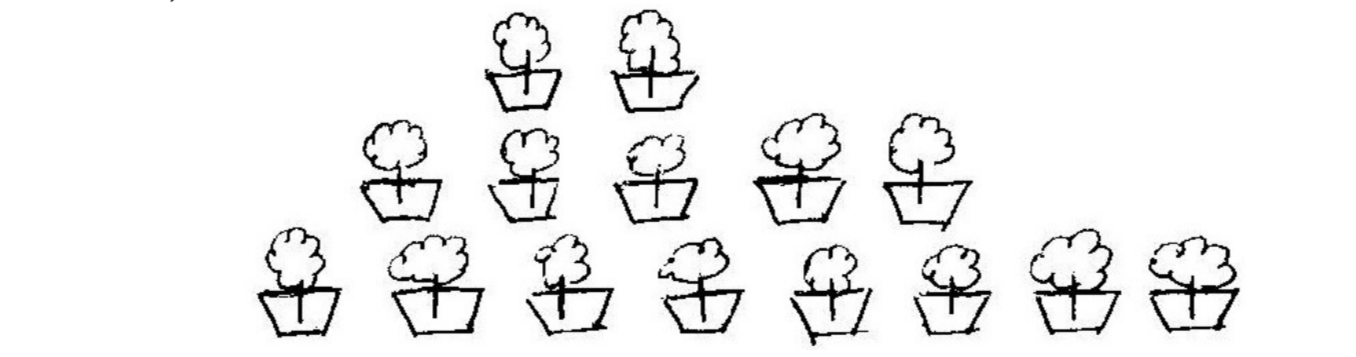
\includegraphics[width=\columnwidth]{figs/ap/Plant.png}
			\caption{Plants}
			\label{fig:Plants}
		\end{figure}
		Based on the above, answer the following questions :
		\begin{enumerate}[label=(\roman*)]
\item How many pots were placed in the $7^{th}$ row ?
				\begin{enumerate}[label=\Alph*]
					 \item $20$
					 \item $23$
					 \item $77$
					 \item $29$
				\end{enumerate}
 \item If Roshini wants to place $100$ pots in total, then total number of rows formed in the arrangement will be ?
				\begin{enumerate}[label=\Alph*]
					 \item $8$
					 \item $9$
					 \item $10$
					 \item $12$
				\end{enumerate}
 \item How many pots are placed in the last row ?
				\begin{enumerate}[label=\Alph*]
					 \item $20$
					 \item $23$
					 \item $26$
					 \item $29$
				\end{enumerate}
			\hfill (2021) \item If Roshini ha sufficient space for $12$ rows, then how many total number of pots are placed by her wih the same arrangement ?
				\begin{enumerate}[label=\Alph*]
					 \item $222$
					 \item $155$
					 \item $187$
					 \item $313$
				\end{enumerate}
		\end{enumerate} 
\hfill (2021)
	 \item The sum of the first $4$ terms of an A.P. is zero and its $4^{th}$ term is $2$. Find the A.P.
	\hfill (2021) \item If the sum of the first $n$ terms of an A.P. is given by $S_n = 4n - n^2$, then find its $n^{th}$ term. Hence, find the $25^{th}$ term and the sum if the first 25 terms of this A.P.
\hfill (2021)
	 \item Find the mean of first $10$ composite numbers.
	\hfill (2021) \item If $S_n$ denotes the sum of first $n$ terms of an A.P., prove that $S_{12} = 3(S_8 - S_4)$.
	\hfill (2021) \item After how many decimal places will the decimal expansion of the rational number $\frac{14587}{1250}$ terminate ?			
\hfill (2021)
	 \item If the $6^{th}$ and $14^{th}$ terms of an A.P. are 29 and 69 respectively, then find the $10^{th}$ term of the A.P.
	\hfill (2021) \item If the first three consecutive terms of an A.P. are $3y-1, 3y+5$ and $5y+1$ find the value of y. 
\hfill (2021)
 \item Which of the following is not an A.P.? 
\begin{enumerate}[label =(\Alph*)]
               \item $-1.2,0.8,2.8,\dots$ 
	        \item $3,3+\sqrt2,3+2\sqrt2,3+3\sqrt2,\dots$ 
	        \item $\frac{4}{3},\frac{7}{3},\frac{9}{3},\frac{12}{3},\dots$ 
	        \item $\frac{-1}{5},\frac{-2}{5},\frac{-3}{5},\dots$ 
\end{enumerate}

\hfill (2020) \item Find the sum of the first $100$ natural numbers.	
	\hfill (2020)
 \item Find the Sum:
\begin{align*}
	\brak{-5} + \brak{-8} + \brak{-11} + \dots + \brak{-230}
\end{align*}
\hfill (2020)

 \item Find the number of terms in the A.P. :
\begin{align*}
    18,15\frac{1}{2},13, ...,-47.
\end{align*}

\hfill (2019) \item Determine the A.P. whose third term is $16$ and $7^{th}$ term exceeds the $5^{th}$ term by $12$.

\hfill (2019) \item Find the value of $x$, when in the A.P. given below
\begin{align*}
2 + 6 + 10 + ... + x = 1800.    
\end{align*}

\hfill (2019) \item Which term of the A.P. $-4, - 1, 2, ... $is$ 101$?

\hfill (2019) \item In an A.P., the first term is $- 4$, the last term is $29$ and the sum of all its terms is $150$. Find its common difference.
\hfill (2019)

\hfill (2019) \item Find the $21^{st}$ term of the A.P. $-4 \frac{1}{2},-3,-1\frac{1}{2},...$

\hfill (2019) \item Find the common difference of the Arithmetic Progression (A.P.) 
\begin{align*}
\frac{1}{a} , \frac{3-a}{3a},\frac{3-2a}{3a} , . . (a \neq 0)
\end{align*}

\hfill (2019) \item Which term of the Arithmetic Progression $-7, -12, -17, -22, ... $ will be $-82$ ? Is $-100$ any term of the A.P. ? Give reason for your answer.

\hfill (2019) \item How many terms of the Arithmetic Progression $45, 39, 33, ... $must be taken so that their sum is $180$ ? Explain the double answer.

\hfill (2019) \item Find after how many places of decimal the decimal form of the number $\frac {27}{2^3.5^4.3^2}$ will terminate.

\hfill (2019) \item Find the sum of first $10$ multiples of $6$

\hfill (2019) \item If $m$ times the $m^{th}$ term of an Arithmetic Progression is equal to $n$ times
its $n^{th}$ term and $m \neq n$, show that the $\brak{m + n}^{th}$ term of the A.P is zero

\hfill (2019) \item The sum of the first three numbers in an Arithmetic Progression is $18$. If the product of the first and the third term is $5$ times the common
difference, find the three numbers.
 \item Find the sum of all the two digit numbers which leave the remainder $2$ when divided by $5$.

\hfill (2019) \item If in an A.P ., $a=15$,$d=-3$ and $a_n=0$, then find the value of $n$.

\hfill (2019) \item If ${S_n}$, the sum of the first ${n}$ terms of an A.P. is given by ${S_n = 2n^2 + n}$,then find its $n^{th}$ term. 

\hfill (2019) \item If the $17^{th}$ term of an A.P. exceeds its $10^{th}$ term by $7$, find the common difference.

\hfill (2019) \item If the sum of the first $p$ terms of an A.P. is $q$ and the sum of the first $q$ terms is $p$; then show that the sum of the first $\brak{p + q}$ terms is $\cbrak {-\brak {p + q}}$.

\hfill (2019) \item Write the common difference of the A.P.${\sqrt3} , {\sqrt12} , {\sqrt27} , {\sqrt48}$ , ... 

\hfill (2019) \item In an A.P., the $n^{th}$ term is ${\frac{1}{m}}$ and the $m^{th}$ term is $\frac{1}{n}$. Find 
\begin{enumerate}
      \item  $\brak{mn}^{th}$term  ,
      \item sum of first $\brak{mn}$ terms.
\end{enumerate}
\hfill (2019)

 \item The first term of an AP is 3, the last term is 83 and the sum of all its terms is 903. Find the number of terms and the common difference of the AP.
\hfill (2019) \item If the sum of first $n$ terms of an $AP$ is $n^2$, then find its $10$th term.
\hfill (2019) \item Which term of the $AP$ $3, 15, 27, 39, ....$ will be $120$ more than its $21$st term?
\hfill (2019) \item If $S_n$ ,the sum of first $n$ terms of an $AP$ is given by $S_n=3n^2-4n$, find the $n$th term.
\hfill (2019) \item If the sum of first four terms of an $AP$ is $40$ and that of first $14$ terms is $280$. Find the sum of its first $n$ terms.
\hfill (2019)

			 \item In an $AP$, if the common difference $(d) = -4$, and the seventh term$(a_7)$ is $4$, then find the first term.		
			\hfill (2018) \item The sum of four consecuive numbers in an AP is $32$ and the ratio of the product of the first and the last term to the product of two middle term is $7:15$. Find the numbers.
	\hfill (2018) \item Find the sum of $8$ multiples of $3$.
\hfill (2018)

			 \item In an $AP$, if the common difference $(d) = -4$, and the seventh term$(a_7)$ is $4$, then find the first term.		
			\hfill (2018) \item The sum of four consecuive numbers in an AP is $32$ and the ratio of the product of the first and the last term to the product of two middle term is $7:15$. Find the numbers.

	\hfill (2018) \item Find the sum of $8$ multiples of $3$.
\hfill (2018)
 \item The $5^{th}$ and $15^{th}$ terms of an A.P. are $13$ and $-17$ respectively. Find the sum of first $21$ terms of the A.P.
\hfill (2018)

 \item The sum of the first $n$ terms of an A.P. is $5n^{2}+3n$. If its $m^{th}$ terms is $168$, find the value of $m$. Also find the $20^{th}$ term of the A.P.
\hfill (2018) \item The $4^{th}$ and the last terms of an A.P. are $11$ and $89$ respectively. If there are $30$ terms in the A.P., find the A.P and its $23^{rd}$ term.
\hfill (2018) \item Write the $m^{th}$ term of the A.P. $\dfrac{1}{k}$,$\dfrac{1+k}{k}$,$\dfrac{1+2k}{k}$,........
\hfill (2018)
\end{enumerate}

